% Copyright 2022 by Marek Rychly <rychly@fit.vut.cz>.
%
\documentclass[10pt,xcolor=pdflatex,dvipsnames,table,oneside]{book}
% babel and encoding
\usepackage[czech]{babel}
\usepackage[T1]{fontenc}
\usepackage[utf8]{inputenc}
\usepackage{lmodern}

\usepackage{csquotes}% correct/formal language-specific quotations
\usepackage{microtype}% character protrusion, font expansion, adjustment of interword spacing, additional kerning, tracking, etc.
\usepackage{hyperref}% hyper-refs in PDF
\usepackage{graphicx}

\author{
    František Koleček, \href{mailto:xkolec08@stud.fit.vut.cz}{xkolec08@stud.fit.vut.cz} \\
    Tomáš Moravčík, \href{mailto:xmorav41@stud.fit.vut.cz}{xmorav41@stud.fit.vut.cz} \\
    David Sladký, \href{mailto:xsladk07@stud.fit.vut.cz}{xsladk07@stud.fit.vut.cz}
    }
\title{Ukládání rozsáhlých dat v NoSQL databázích}
\date{zima 2022}

\begin{document}

\pagenumbering{roman}

\hypersetup{pageanchor=false}% disable hyperref anchor to title page as maketitle enforce pagenumbering to arabic which colides the titlepage with the first arabic page below
\maketitle
\hypersetup{pageanchor=true}

\tableofcontents

\newpage% force page-break to start the page numbering on a new page
\pagenumbering{arabic}

\part{Analýza zdrojových dat a návrh jejich uložení v NoSQL databázi}

\chapter{Analýza zdrojových dat}

Použitá datová sada se nachází na stránkách \href{https://mdcr.cz/Dokumenty/Verejna-doprava/Jizdni-rady,-kalendare-pro-jizdni-rady,-metodi-%281%29/Jizdni-rady-verejne-dopravy}{ministerstva dopravy}
a to konrétně \href{https://portal.cisjr.cz/pub/draha/celostatni/szdc/}{zde}. Detailní popis formátu dokumentů datové sady lze najít na stejném \href{https://portal.cisjr.cz/pub/draha/celostatni/szdc/Popis%20DJ%C5%98_CIS_v1_09.pdf}{místě}.

Datová sada se skládá z \verb|XML| souborů. Tyto soubory jsou zveřejňovaný na začátku roku pro celý rok ve složce \verb|GVD|. Dále je pak každý měsíc zveřejňována datová sada pro daný měsíc s aktualizacemi pro spoje.
Každý soubor má element \verb|CZPTTCreation|, který určuje jeho vytvoření.

\verb|XML| soubory lze rozdělit do následujících tří skupin:
\begin{itemize}
    \item Definující spoj
    \item Rušící spoj
    \item Definující náhradní spoj
\end{itemize}
Soubory definující spoje mají jako kořenový element \verb|CZPTTCISMEssage|. První důležité informace se nachází v elementu \verb|Identifiers|,
kde jsou uvedeny identifikátory pro definované spojení a vlak, který ho bude provádět. Dále element \verb|CZPTTHeader| určuje, zda spoj
přijíždí nebo pokračuje z/do zahraniční stanice. Elementy \verb|CZPTTLocation| obsahují jednotlivé stanice, kterýma vlak projiždí. Zde jsou
uvedeny i další informace ke stanici. Nejvýznamnější z nich jsou: čas příjezdu/odjezdu, typ aktivity. Po uvedení všech stanic následuje
element \verb|PlannedCalendar|, který určuje výčet dní, kdy je tento spoj prováděň.

Soubory rušící spoje mají kořenový element \verb|CZCanceledPTTMessage|. Podobně jako soubory definující spoje obsahují identifikaci spoje, který se ruší
a výčet dní, kdy se ruší. Dále už nenesou žádné informace.

Soubory definující náhradní spoje mají stejnou strukturu jako soubory definující spoje jenom s jediným rozdíle. Obsahují element
\verb|RelatedPlannedTransportIdentifiers|, který určuje, jaký spoj nahrazují. Tyto spoje mají unikátní indentifikátor vůči
normálním spojům.

\chapter{Návrh způsobu uložení dat}
\section{Definice entit a vazeb mezi nimi}
Z datové sady poskytnuté XML soubory lze definovat několik entit a vazeb mezi nimi vhodných pro uložení do NoSQL databáze.
\subsection{File}
Samotné soubory lze považovat za entity pro uložení. Tyto entity ponesou informace o jméně souboru,
který reprezentují a času, kdy byl soubor vytvořeny z elementu CZPTTCreation.

\vspace{1em}
\begin{tabular}{|l|}
    \hline
    :File \\
    \hline
    filename \\
    creation \\
    \hline
\end{tabular}

\subsubsection{PRECEDES}
Novější soubory aktualizují stav definovaný předcházejícími soubory, proto mezi jednotlivými entitami :File
budou vazby :PRECEDES, které spojí soubor s jeho nejbližším následníkem.

\vspace{1em}
\begin{tabular}{|l|}
    \hline
    :File \\
    \hline
\end{tabular}
\begin{tabular}{c}
    -- :PRECEDES --> \\
\end{tabular}
\begin{tabular}{|l|}
    \hline
    :File \\
    \hline
\end{tabular}

\subsubsection{DEFINES}
Pokud se nejedná o soubor rušící spoj, tak tento soubor definuje o jakém spoji podává informace. Tuto vlastnost bude modelována vazbou :DEFINES.

\vspace{1em}
\begin{tabular}{|l|}
    \hline
    :File \\
    \hline
\end{tabular}
\begin{tabular}{c}
    -- :DEFINES --> \\
\end{tabular}
\begin{tabular}{|l|}
    \hline
    :PA \\
    \hline
\end{tabular}

\subsubsection{CANCELS}
Pokud se jedná o soubor rušící spoj, tak tento soubor definuje jakého spoje ruší jízdy. Tuto vlastnost bude modelována vazbou :CANCELS.

\vspace{1em}
\begin{tabular}{|l|}
    \hline
    :File \\
    \hline
\end{tabular}
\begin{tabular}{c}
    -- :CANCELS --> \\
\end{tabular}
\begin{tabular}{|l|}
    \hline
    :PA \\
    \hline
\end{tabular}

\subsection{PA}
Další významnou entitou jsou spoje. Tyto spoje budou označovány jako PA -- stejně jako v souborech v elementu Object Type.

\vspace{1em}
\begin{tabular}{|l|}
    \hline
    :PA \\
    \hline
    Core \\
    Company \\
    Variant \\
    TimetableYear \\
    NetworkSpecificParameters \\
    Header \\
    \hline
\end{tabular}

\subsubsection{SERVER BY}
Každý spoje je prováděn vlakem. Tento vlak je vždy uveden v souboru se spojem, který provádí. Tuto vlastnost
definujeme jako :SERVED BY.

\vspace{1em}
\begin{tabular}{|l|}
    \hline
    :PA \\
    \hline
\end{tabular}
\begin{tabular}{c}
    -- :SERVED BY --> \\
\end{tabular}
\begin{tabular}{|l|}
    \hline
    :TR \\
    \hline
\end{tabular}

\subsubsection{RELATED}
Pokud se jedná o spoj, který nahrazuje jiný spoj, tak je také definováno jaký spoj je nahrazován. Tuto vlastnost
modelujeme jako :RELATED.

\vspace{1em}
\begin{tabular}{|l|}
    \hline
    :PA \\
    \hline
\end{tabular}
\begin{tabular}{c}
    -- :RELATED --> \\
\end{tabular}
\begin{tabular}{|l|}
    \hline
    :PA \\
    \hline
\end{tabular}

\subsubsection{GOES IN}
U každého spoje je také uvedeno, v jaké dny jezdí. Informaci v jaké dny jeden reprezentujeme vazbou :GOES IN mezi spojem a dnem.

\vspace{1em}
\begin{tabular}{|l|}
    \hline
    :PA \\
    \hline
\end{tabular}
\begin{tabular}{c}
    -- :GOES IN --> \\
\end{tabular}
\begin{tabular}{|l|}
    \hline
    :Day \\
    \hline
\end{tabular}

\subsubsection{IS IN}
Každý spoj projíždí minimálně dvěmi stanicemi. Tuto vlastnost modelujeme vztahem :IS IN mezi spojem a stanicí.
Tato vazbna také neve řadu parametrů definující příjez, odjezd, prováděné akce a podobné.

\vspace{1em}
\begin{tabular}{|l|}
    \hline
    :PA \\
    \hline
\end{tabular}
\begin{tabular}{c}
    -- :IS IN --> \\
\end{tabular}
\begin{tabular}{|l|}
    \hline
    :Station \\
    \hline
\end{tabular}

\vspace{1em}
\begin{tabular}{|l|}
    \hline
    :IS IN \\
    \hline
    LocationSubsidiaryCode \\
    AllocationCompany \\
    LocationSubsidiaryName \\
    ALA \\
    ALAOffest \\
    ALD \\
    ALDOffset \\
    DwellTime \\
    ResponsibleRU \\
    ResponsibleIM \\
    TrainType \\
    TrafficType \\
    CommercialTrafficType \\
    TrainAvtivityType \\
    OperationalTrainNumber \\
    NetworkSpecificParameters \\
    \hline
\end{tabular}

\subsection{TR}
Soubory jsou také definovány vlaky, které provádí spoje. Tyto vlaky budou znázorněny entitami :TR.

\vspace{1em}
\begin{tabular}{|l|}
    \hline
    :TR \\
    \hline
    Core \\
    Company \\
    Variant \\
    TimetableYear \\
    NetworkSpecificParameters \\
    \hline
\end{tabular}

\subsection{Station}
V XML souborech jsou také definováné stanice, kterými vlak projíždí. Tyto stanice budou modelovány pomocí
entit :Station.

\vspace{1em}
\begin{tabular}{|l|}
    \hline
    :Station \\
    \hline
    LocationPrimaryNumber \\
    PrimaryLocationName \\
    CountryCodeISO \\
    \hline
\end{tabular}

\subsection{Day}
U každého spoje je také určeno, v jaké dny jezdí. Tyto dny budou existovat jeko entity :Day.

\vspace{1em}
\begin{tabular}{|l|}
    \hline
    :Day \\
    \hline
    Date \\
    \hline
\end{tabular}

\begin{figure}
    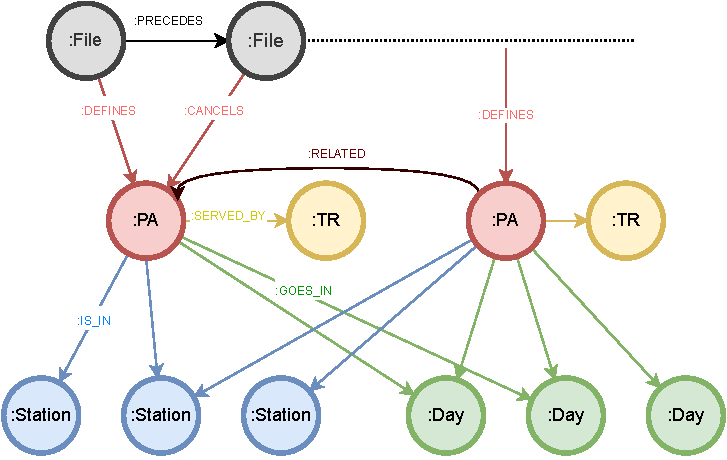
\includegraphics[width=1\textwidth, angle=0]{img/structure.pdf}
    \caption{Finální schéma entit a vazeb meiz nimi v databázi.}
\end{figure}

\chapter{Zvolená NoSQL databáze}
Pro řešení tohoto problému jsme zvolili grafovou databázi, konkrétně \href{https://neo4j.com/}{Neo4j}. Grafová databáze nám umožní
reprezentovat entity jako uzly v grafu a vztahu mezi entitaby jako cesty mezi těmito uzly. Zároveň je možné u uzlů i
cest definovat další vlastnosti typu klíč:hodnota, co zase umožní uložit veškeré další potřebné informace
vztahující se k jednotlivým objektům. Neo4j poskytuje webové rozhraní pro databázi, které umožňuje jednoduché
zadávání požadavků na databázi. S kombinací s tím, že toto webové rozhraní také zobrazuje získané výsledky do
grafu, tak nám to umožní snadnější opravování chyb v aplikaci a snadnější vytváření potřebných požadavků na databázi.

\part{Návrh, implemetace a použití aplikace}

\chapter{Návrh aplikace}
\iffalse
\paragraph{Cíl:}
Navrhnout hlavní části aplikace splňující požadavky zadání s důrazem na práci s na ni napojenou databází NoSQL či datovými zdroji
(při jejich předzpracování a nahrávání do NoSQL databáze).

\paragraph{Obsah:}
Použité technologie (např. skriptovací jazyk, knihovny, atp.)
a architektura (např. skript či sekvence skriptů pravidelně spouštěných v daných časových intervalech či v reakci na danou událost).
Způsob technického řešení úloh ze zadání (jejich průběh v aplikaci) a konceptů z předchozího návrhu (struktury, algoritmy, toky dat, atp.).

\paragraph{Prostředky:}
Strukturovaný text (sekce, odstavce, odrážky, atp.), případně pseudokód či obrázky, doplňující technické detaily konceptů nastíněných v předchozím návrhu.
Důraz je kladen na způsob realizace dotazů ze zadání.

\paragraph{Fáze projektu:}
Návrh aplikace a částečně po či souběžně s návrhem databáze.
\fi
\section{Zpracování souborů XML}

Informace o vlakových spojích jsou získávány ze souborů ve formátu XML. Tyto soubory je třeba zpracovat – nahrát data do strukturované vnitřní reprezentace programu, pro efektivní nahrávání do databáze. Každý soubor obsahuje informace o jednom konkrétním vlakovém spoji, jeho cesta a časy ve stanicích jsou vždy stejné, jsou zde definované dny, ve kterých tento spoj jede. Nejdůležitější zpracovávaná data jsou:

\begin{itemize}
    \item Identifikátory
    \item Navštívené stanice a časy příjezdu a odjezdu
    \item Dny, ve kterých spoj jede
\end{itemize}

\subsection{Struktura XML souborů}
Každá s těchto informací se nachází ve vlastní „větvi“ v souboru. Nachází se u nich samozřejmě i dodatečné informace – detaily lokace, činnost vlaku ve stanici atd. Platné dny jsou určeny pomocí dvou atributů – začátek a konec platnosti a bitmapa. Bitmapou je myšlen řetězec jedniček a nul, kde jedničky vyjadřují platnost v jednotlivých dnech. Tímto způsobem lze vyjádřit platné dny na rok dopředu pomocí řetězce dlouhém 365 znaků.

\subsection{Zvolené Prostředky}
Zpracovávání souborů je implementováno v jazyce Python v souboru \verb|parser.py|. Je využito modulu \verb|xml|, který je součástí základní instalace Pythonu, není třeba jej dodatečně instalovat. Tento modul obsahuje třídu \verb|ElementTree|, která umožňuje snadné nahrávání dat ze stromové struktury souboru. Velmi užitečnou funkcí je možnost adresování uzlů pomocí „cesty“ - obdobným způsobem jako adresování souborů v souborovém systému.

\subsection{Způsob implementace}
Nejdůležitější roli při zpracovávání hraje funkce \verb|node_to_dict|, která rekurzivně prohledává daný uzel a převádí jeho obsah na slovníkový datový typ.

Protože platné dny jsou v naší databázi ukládány jako vlastní uzly, na které pak odkazují spoje, které jsou platné v daný den, je potřeba původní reprezentaci platných dní (popsána výše) převést na seznam konkrétních kalendářních dat. Pro implementaci této funkcionality byl využit modul \verb|datetime|, který je opět součástí základní instalace pythonu. Tento modul mimo jiné umožňuje vykonávat „aritmetické operace“ s kalendářními daty. V našem případě se jedná o sečtení data začátku platnosti a indexu jedničky v příslušné bitmapě. Implementace je ve funkci \verb|cal_to_listofdays|.

\chapter{Způsob použití}

\paragraph{Cíl:}
Poskytnout stručnou dokumentaci pro zprovoznění databáze a aplikace.

\paragraph{Obsah:}
Stručně popsat, jak celé řešení zprovoznit, tj. nasadit databázi i aplikaci vč. způsobu volání aplikace (příkazový řádek, parametry) pro úlohy
předzpracování a nahrání dat ze zdroje do databáze a pro ulohy hledání nad databází tak, jak byly definovány v zadání.

\paragraph{Prostředky:}
Stručný text obsahující návod (popis) s ukázkami způsobu volání aplikace (např. pro skripty by to byl kód příkazového řadku).

\paragraph{Fáze projektu:}
Dokončování implementace, chystání dokumentace pro předání výsledného systému zákazníkovi.

\chapter{Experimenty}

\paragraph{Cíl:}
Změřit, jak aplikace a databáze fungují v praxi.

\paragraph{Obsah:}
Popis výchozí konfigurace aplikace a nasazení databáze stroje, kde budou experimenty probíhat (HW a SW).
Popis experimentů typicky představující nahrání dat ze zdroje do databáze či dotazy ze zedání s výslednými časy jejich provedení.
Případné poznámky k výsledkům experimentů.

\paragraph{Prostředky:}
Strukturvaný text, případně tabulka či graf s doprovodným textem.

\paragraph{Fáze projektu:}
Testování řešení před předáním výsledného systému zákazníkovi.

\section{Rychlost zpracování XML souborů}
Funkčnost a efektivita skriptu \verb|parser.py| byla testována nad složkou \verb|GVD2022|, která obsahuje přibližně 12300 souborů formátu XML. Všechny soubory byly v experimentu zpracovány a výpis důležitých informací vytisknut na standardní výstup. Tato operace trvala 93 sekund, tedy cca 132 zpracovaných souborů za sekundu.

\end{document}
